\documentclass[12pt,a4paper]{jbook}
\usepackage{mm-thesis}
\usepackage[dvipdfmx]{graphicx}
\usepackage{cite}
\usepackage{comment}
\usepackage{docmute}
\usepackage{color}
\usepackage{moreverb}
\usepackage{listings}
\usepackage{ascmac}
%\usepackage{amsmath}
%\usepackage{amsthm}
%\usepackage{amsfonts}

\lstset{
	%枠外での自動改行
 	breaklines = true,
 	%標準の書体
 	basicstyle = {\small},
 	%枠 "t"は上に線を記載, "T"は上に二重線を記載
	%他オプション:leftline,topline,bottomline,lines,single,shadowbox
 	frame = TB,
 	%タブの大きさ
 	tabsize = 2,
 	%キャプションの場所("tb"ならば上下両方に記載)
 	captionpos = t,
 	%行番号の位置
 	numbers = left,
 	%自動改行後のインデント量(デフォルトでは20[pt])	
 	breakindent = 30pt,
	%左右の位置調整 	
 	xleftmargin=30pt,
 	xrightmargin=30pt,
	%プログラム言語(複数の言語に対応,C,C++も可)
 	%language = Python, 	
 	%背景色と透過度
 	%backgroundcolor={\color[gray]{.90}},
 	%コメントの書体
 	%commentstyle = {\itshape \color[cmyk]{1,0.4,1,0}},
 	%関数名等の色の設定
 	%classoffset = 0,
 	%キーワード(int, ifなど)の書体
 	%keywordstyle = {\bfseries \color[cmyk]{0,1,0,0}},
 	%表示する文字の書体
 	%stringstyle = {\ttfamily \color[rgb]{0,0,1}},
 	%frameまでの間隔(行番号とプログラムの間)
 	%framesep = 5pt,
 	%行番号の間隔
 	%stepnumber = 1,
	%行番号の書体
 	%numberstyle = \tiny,
}
\renewcommand{\lstlistingname}{Code}
\begin{document}
\newpage

\chapter{提案モデル}
この章では、ウェブの様々な要素に利用可能なAlloyでの時相論理の記述法と、その応用例としてキャッシュを実装したウェブセキュリティモデルを提案する。

\section{汎用的な時相論理のAlloy上の記述法の提案}
\label{sec:ProposedModel-TemporalLogic}
前述の\ref{sec:existing-models-problems}節における既存モデルの時相論理の表現能力の問題点は、「時間軸全体を通して状態変化を追うことができない」ことである。
そもそも、既存モデルが同一のTransaction間の状態変化のみの表現能力となっているのは、状態を表すクラス(CookieモデルにけるCSStateクラス)間の時間軸上での順序の表現を、ツールの機能を利用しない論理式で実現することが難しいためである。
したがって、状態を表すクラス間の時間軸上の関係性を表現できる述語が必要となる。
また、CookieモデルにおけるCSStateクラスはCookieの状態を表現するためのクラスであり、CSStateのみに利用できる述語では今後の他のウェブの要素に利用できない。
以上より、様々なウェブの要素の状態を表現するための汎用的なクラスを定義し、そのクラスに利用可能な述語を作成する。

また、時間軸全体を通して状態変化を表現するためには必要となる述語を考える。
まず、ある状態からその直前の状態を判定できれば、「前後の二状態で起こりうる変化」を表現可能になる。
これに加えて状態遷移の初期状態を判定できれば、「初期状態にかかる条件(初期条件)」を表現可能になる。
これら二つの表現能力を組み合わせることで、帰納的に時間軸全体で起こりうる状態変化を表現可能となる。
したがって、これらの表現能力を実装するため、以下の述語を作成する。
\begin{itemize}
\item Transactionの関係に関わらず、直前にあたる状態を判定する述語
\item 初期状態を判定する述語
\end{itemize}

また、本記述法を用いる上で基礎モデルでの時間軸の表現(\ref{sec:based-model-temporal-logic}節参照)を一部変更している。
その変更点についても以降で述べる。

\subsubsection{時間軸の表現の変更}
基礎モデル\cite{based-model}においては、時間軸を表すTimeクラスにネットワーク上で発生するレスポンスやリクエストを表すEventクラスが関連付けられている。
これらのクラス間の関係性は、「ある時点Time0とTime1の間でEvent0が発生した」といった内容を表現できるというものであり、二つのTimeクラスのインスタンスで一つのイベントの時刻を表現できる。

しかし、本提案モデルではEventクラスに加えて、ある時点におけるウェブの要素の状態を表すStateクラスも時間軸に関連付けられる。
ここで、二つのTimeクラスのインスタンスで一つのイベントの時刻を表現するという既存モデルの関係性を維持すると、導入する述語の論理式が複雑となり実装が困難となる。
したがって、本提案モデルでは図\ref{fig:ProposedModel-TimeClass}に示す、一つのTimeクラスのインスタンスでイベントの時刻を表現できる記述法に変更する。

\begin{figure}[htb]
\centering
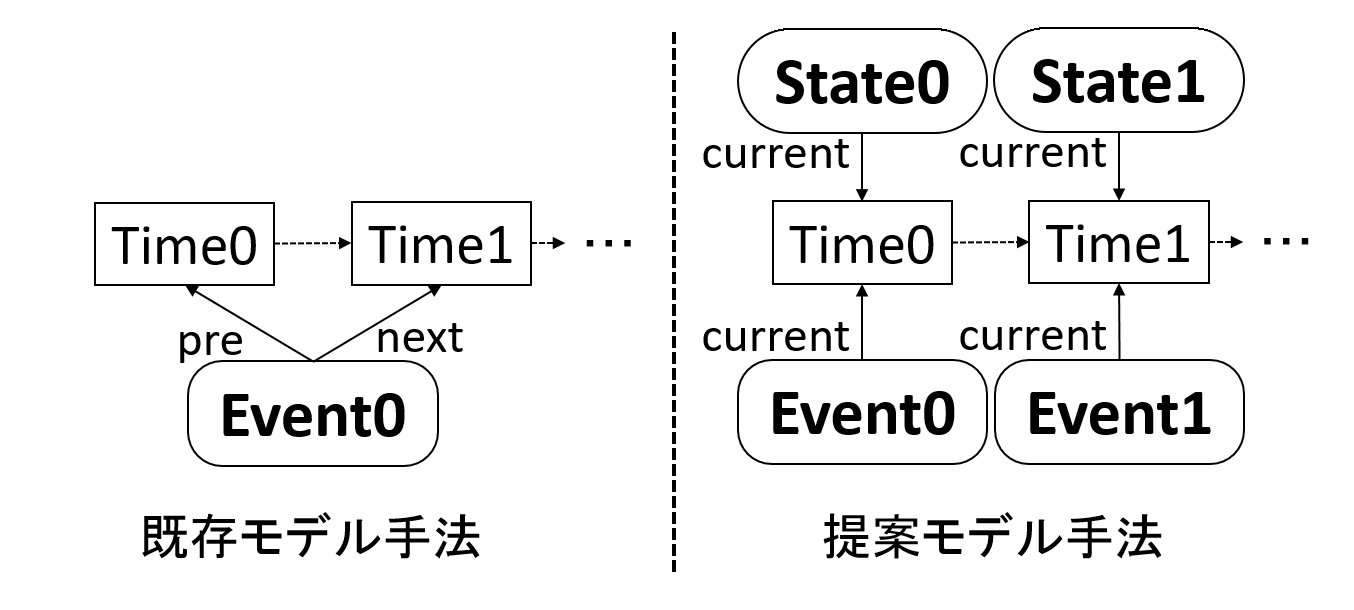
\includegraphics[width=450pt]{./fig/ProposedModel-TimeClass.eps}
\caption{提案モデルにおける時間軸とイベントの関係}
\label{fig:ProposedModel-TimeClass}
\end{figure}

この記述の変更によって、二つの既存モデルそれぞれにおける時相論理の表現能力に変更はない。
そもそも、基礎モデルで二つのTimeクラスのインスタンスを利用する関係性とした理由は、今後の拡張において「リクエストやレスポンスといったイベントが同時刻で発生しない」という基礎モデルの制限を無くすことを想定したためである。
本提案モデルにおいてもこの制限事項は継承しているが、一つのTimeクラスのインスタンスによる表現としたとしても、同じTimeクラスのインスタンスとの関係を持つEventクラスのインスタンスが複数存在することを許容することで今後の拡張は可能である。
つまり、この変更によって既存モデルの表現能力と拡張性を妨げない。

\subsubsection{状態を表現する汎用クラス}
導入する汎用クラスとしてCode\ref{code:StateClass}に示すStateクラスを定義する。
flowはStateクラス同士を接続し状態の遷移を、currentはその状態となり得る時刻を表す。
また、その他の項目としてEqItem、DifItemクラスをStateクラスの変数としている。
\begin{lstlisting}[caption=Stateクラス, label=code:StateClass]
abstract sig State{
	flow: set State,
	eq: one EqItem,
	dif: one DifItem,
	current: set Time
}
abstract sig EqItem{}
abstract sig DifItem{}
sig StateTransaction extends HTTPTransaction{
	beforeState: set State,
	afterState: set State
}
\end{lstlisting}

まず、EqItemは同一の状態遷移上で変化しない要素(以下、「一致要素」とする)を表すクラスである。
一致要素は複数のStateが存在する場合に、いずれのStateが同一の遷移であるのかを判定するために必要である。
例えばStateが三つ存在している場合を考えると、図\ref{fig:ProposedModel-3StateFlow}に挙げられるように複数の遷移のパターンが考えられる。
ここで、EqItemをStateごとに比較をすることで、同一のEqItemを持つStateを同一の遷移に存在すると判定することができる。
図\ref{fig:ProposedModel-3StateFlow}を例にとると、三状態が同一の遷移に存在する場合にはState0,1,2のEqItemがすべて同じとなる。
一方で、三状態が同一の遷移に存在しない場合にはState0,2のEqItemが同じであり、State1のEqItemはそれと異なる。

\begin{figure}[htb]
\centering
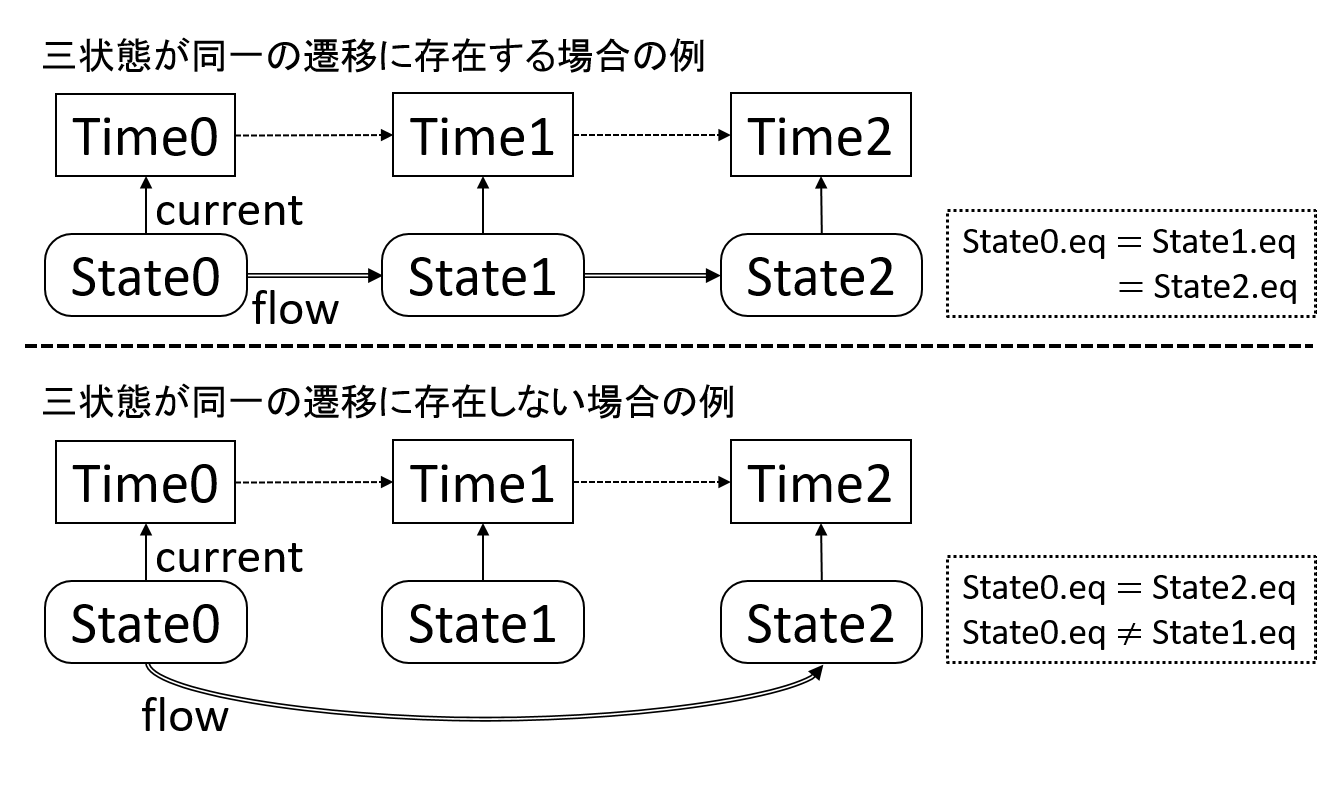
\includegraphics[width=400pt]{./fig/ProposedModel-3StateFlow.eps}
\caption{3状態間における遷移の一例}
\label{fig:ProposedModel-3StateFlow}
\end{figure}

また、DifItemは状態遷移において変化する要素(以下、「変化要素」とする)を表すクラスである。
状態変化をモデルで表現した際に捉えたい項目をDifItemに記述する。

最後に、これらのStateはCookieモデルと同様にHTTPTransactionに関連付けることで、レスポンスとリクエスト時の状態を表す。
したがって、HTTPTransactionを継承しStateクラスを持つStateTransactionをCode\ref{code:StateClass}の9-12行目で定義している。

このStateクラスを利用してウェブの要素の状態遷移を考えるには、State、EqItem、DifItemクラスを継承するその要素専用のクラスを定義する。
また、その要素について一致要素と変化要素を明らかにしておき、継承後のクラスに記述する。
以下のCode\ref{code:CookieClass}はCookieモデルを基にしたCookieへの応用例である。
2,3行目に記すように、Stateを継承するクラスではeqとdifもまた、EqItem、DifItemを継承する専用のクラスに含まれるように条件を記述する。
Cookieモデルでは、一致要素がクライアント、変化要素がCookieの集合となっている。
これは、各クライアント毎にでCookieの保存が行われているため、状態遷移の上でクライアントは変更されないためである。
また、変化要素は変化を捉えたい要素である、クライアント内で保存されているCookieを表現している。
\begin{lstlisting}[caption=Cookieへの応用例, label=code:CookieClass]
sig CookieState extends State{}{
	eq in CookieEqItem
	dif in CookieDifItem
}
sig CookieEqItem extends EqItem{
	client: one HTTPClient
}
sig CookieDifItem extends DifItem{
	cookie: set Cookie
}
\end{lstlisting}

\color{red}
\subsubsection{直前状態を判定する述語}
上記のStateクラスに対して、状態遷移上で直前となる状態を判定する述語JustBeforeStateを利用できる(Code\ref{code:JustBeforeState}参照)。
このJustBeforeStateは三つの引数を要する。
そのうちの二つはStateクラスでありそれぞれpre、postと表す。
述語JustBeforeStateはpreがpostの直前の状態であるか考える。
しかし、postが複数の時刻を持つ場合があり、この場合には二つのStateの入力では複数の組み合わせで真となる。
そこで、postの時刻を指定するため、StateTransactionを引数に追加する(これをstrとする)。
これにより、与えられたトランザクションに含まれるpostの時刻に限定して、その時刻においてpreが直前であるか判定でき、真となる組み合わせが一意に定まる。
\begin{lstlisting}[caption=状態遷移において直前の状態を判定する述語, label=code:JustBeforeState]
pred JustBeforeState[pre:State, post:State, str:StateTransaction]{
	pre.eq = post.eq
	post in str.(beforeState + afterState)

	some t,t':Time |
		{
			t in pre.current
			t' in str.(request + response + re_res).current
			t' in str.request.current implies post in str.beforeState
			t' in str.(response + re_res).current implies post in str.afterState
			t' in t.next.*next

			all s:State, t'':Time |
				(s.eq = pre.eq and t'' in s.current) implies
						(t in t''.*next) or (t'' in t'.*next)
		}
}
\end{lstlisting}

また、この述語JustBeforeStateが真となる条件は以下の三つに分割でき、引数がすべてを満たす場合に述語JustBeforeStateも真となる。
\begin{itemize}
\item preとpostの一致要素が同一であること(2行目)
\item postがstrのbeforeState、afterStateのいずれかに属していること(3行目)
\item preの時刻とpostのstrにおける時刻の間の時刻を持つ、一致要素が同一の他の状態が存在しないこと(5-16行目)
\end{itemize}

\subsubsection{初期状態を判定する述語}
Stateクラスに対して利用可能な、もう一方の述語は初期状態を判定する述語FirstStateである(Code\ref{code:FirstState}参照)。
引数としてStateクラスが与えられ(これをsとする)、それが初期状態であるか判定する。
また、一致要素が異なると状態変化がそれぞれ独立するため、それぞれに対して初期状態が生じる。
\begin{lstlisting}[caption=状態遷移において初期状態を判定する述語, label=code:FirstState]
pred FirstState[s:State]{
	all s':State |
		s.eq = s'.eq implies
			s'.current in s.current.*next
}
\end{lstlisting}
\color{black}

\section{提案記述法を用いたキャッシュの実装}
\section{中継者の実装}
\section{提案モデルの制限事項}

\end{document}
